\documentclass{article} % For LaTeX2e
\usepackage{hyperref}
\usepackage{url}
\usepackage[utf8]{inputenc}
\usepackage{amsmath}
\usepackage[numbers,sort]{natbib}
\usepackage{graphicx}
\usepackage[export]{adjustbox}
\usepackage{cleveref}
\usepackage{footmisc}
\usepackage[section]{placeins}
\usepackage{hyperref}
\DeclareGraphicsExtensions{.pdf,.png,.jpg,.eps}

\newlength\tindent
\setlength{\tindent}{\parindent}
\setlength{\parindent}{0pt}
\renewcommand{\indent}{\hspace*{\tindent}}


\author{
Gabriel C-Parent\\
}


\newcommand{\fix}{\marginpar{FIX}}
\newcommand{\new}{\marginpar{NEW}}

\begin{document}


\title{IFT6751: Homework 3}
      
\maketitle
\section{Introduction}

In this homework, an Elastic Net algorithm is used to solve the traveling salesperson problem.

\subsection{The TSP}

The Traveling Salesperson Problem (TSP) is a landmark problem in combinatorial optimization and an hard one (NP-Hard)\citep{euc_tsp_complete}.\newline

The basic idea is that a salesperson needs to travel to a set of cities and come back to its original city in the shortest time (distance) possible. This corresponds to finding an Hamiltonian cycle of minimal distance.\newline

There exists a number of variants of the classical statement such as the metric TSP, euclidean TSP and the asymmetric TSP. 



\subsection{Elastic Net}

The TSP has been studied extensively and many approaches are available to solve it ranging from heuristics to exact methods. The problem was even solved with DNA computing \citep{adleman}. The problem can be formulated as an integer linear program so that classical mathematical programming tools can be used.\newline

The Elastic Net is a geometrical approach to the TSP \citep{en_original}. It consists of having a ring of neurons initialized in the center of the cities which is then elongated (think of a rubber band) by minimizing the length of the band and the distance of the band points to cities for a set number of iterations. Eventually, the rubber band stabilizes and a traversal is extracted by assigning cities to the nearest neuron until no city is left unassigned.\newline

The implementation used here is quite naive and some specifics must be documented. First, every problem instance is transposed onto the unit square to avoid underflow errors. Second, the update rule used here is the same as in \citep{en_original}, that is the parameter K is set to 0.2 and is decreased by 1\% every 25 iterations.

Also, an additional 2-opt descent optimization was performed on the solutions.


\subsection{Evaluation}

From the evaluation standpoint, two relatively easy measures are available: using known problems or generating new ones as in \citep{en_original}.


\subsubsection{TSPLIB instances}

The first way of evaluating the quality of generated solutions is to use previously solved problem instances. To do so, the 2D euclidean TSP instances ("EUC\_2D") from TSPLIB \citep{tsplib} are used. Interestingly, to avoid floating-point precision problems, the total distance are calculated by rounding the distances between cities to the nearest integer.


\subsubsection{Random Problems}
Another way to evaluate the performance of our solver is to simply generate random new instances of problems with fixed number of clients (in this case 50, 100, 200) distributed uniformly through the unit square.

For each problem size, the best distance over 5 different randomly generated instances is reported \citep{en_original}. Obviously, this is done using floating-point distance calculation.




\newpage
\section{Experimental Results}
\label{results}


\subsection{TSPLIB Instances}
First of all, the Elastic Net was used to solve some of the 2D euclidean instances from TSPLIB.

\begin{figure}[!htb]
	\begin{center}
	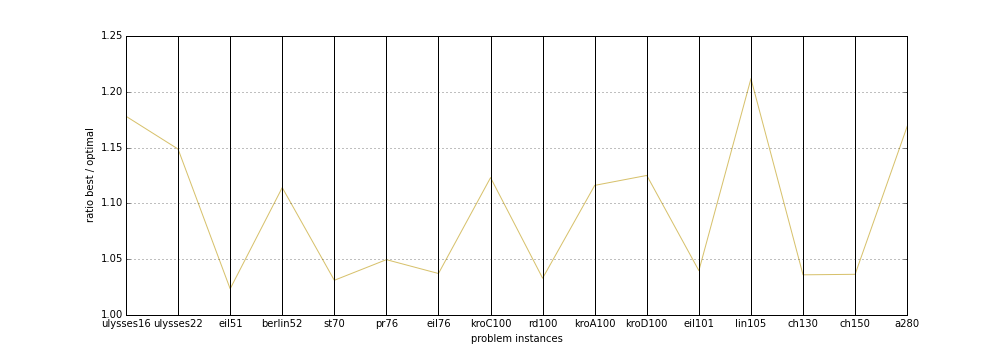
\includegraphics[scale=0.4]{figs/ratios}
	\caption{\small Distance ratio of obtained solution against optimal known solution. The problems are arranged by the number of clients to visit in increasing order from left to right. We can see that the number of clients doesn't seem to influence the relative performance. Full solutions can be visualized in \cref{TSPLIB_solutions}.}
	\end{center}
\end{figure}



\begin{figure}[!htb]
\begin{center}
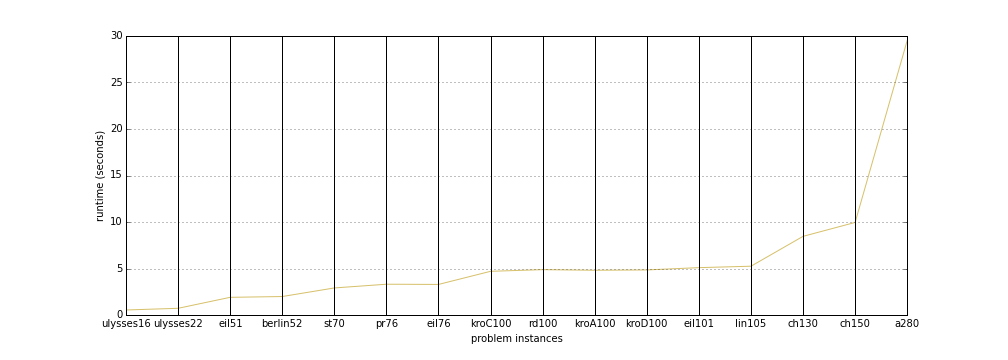
\includegraphics[scale=0.4]{figs/runtimes}
\caption{\small Runtime measured in seconds for the different problem instances. The problems are arranged by the number of clients to visit in increasing order from left to right. We can see that the runtime grows with the number of clients (as expected).}
\end{center}
\end{figure}



\newpage
\subsection{Randomly Generated Instances}

Here are the best results obtained for randomly generated problems of size 50, 100 and 200.

\begin{figure}[!htb]
\begin{center}
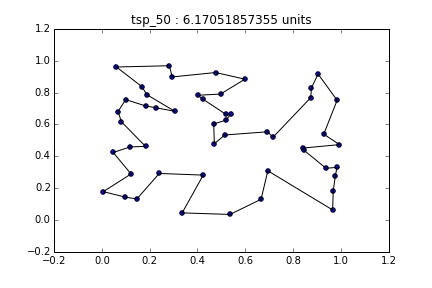
\includegraphics[scale=0.45]{figs/random_tsp_50}
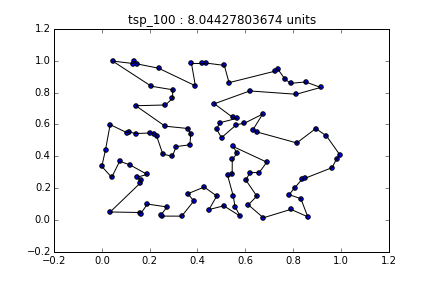
\includegraphics[scale=0.45]{figs/random_tsp_100}
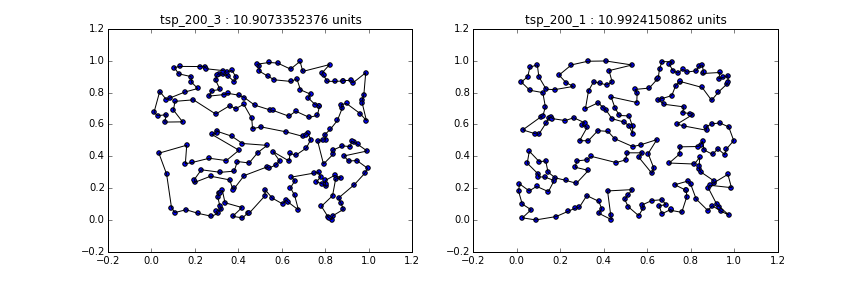
\includegraphics[scale=0.45]{figs/random_tsp_200}

\caption{\small Best solutions to (five different) randomly generated 2D euclidean TSP instances of size 50, 100 and 200. Compared to the results from \citep{potvin_ann}, the results are slightly worse than the ones for the Elastic Net but still much better than the Peterson and Soderberg model results.}
\end{center}
\end{figure}







\newpage
\section{Discussion}
\label{discussion}


\subsection{Implementation details}

The Elastic Net was implemented in a sequential fashion.


\subsection{Challenges}

One needs to avoid exponentiating big negative numbers.


\subsection{Performance}


\subsubsection{Time}

As expected, the algorithm is quite fast and could be much faster given a parallel implementation.


\subsubsection{Quality}

The performance is a bit lower than expected but the results are quite sensitive to parameters.





\section{Conclusion}
\label{conclusion}

The elastic net approach to the TSP is an interesting idea with some nice theoretical guarantees \citep{en_theoretical_analysis}. 



\bibliographystyle{plain}
\bibliography{dev3}


\newpage
\section{Supplementary Materials}

\subsection{User Guide}
\label{user_guide}

The following section should help with verification of the results and repeatability.\newline

The language used is a mix of python and cython, an optimising compiler that allows static typing and generates C code.


\subsubsection{Working Environment}
All computational results obtained in this work should be repeatable given a suitable python environment. The particular dependencies of this work are the Cython, Numpy, IPython and Seaborn along with standard python environment.\newline

The following python environment was used:

\begin{verbatim}
CPython 2.7.9
ipython 2.2.0

numpy 1.9.2
cython 0.21
ipython 2.2.0
seaborn 0.5.1

compiler   : GCC 4.4.7 20120313 (Red Hat 4.4.7-1)
system     : Linux
release    : 3.13.0-46-generic
machine    : x86_64
processor  : x86_64
CPU cores  : 4
interpreter: 64bit

\end{verbatim}

As of now, my personal recommendation is to use the excellent \href{http://continuum.io/downloads}{Anaconda python distribution} from Continuum Analytics.


\subsubsection{Running Computational Results}

All computational results and figures are contained in the form of IPython Notebooks with the hope of allowing repeatability and reproducibility.


If IPython is available on the computer, an IPython Notebook service can be launched from command line using the following call.


This allows viewing and recomputation of the results.\newline


Alternatively, the IPython notebooks can be viewed online if it is reachable from a url using the \href{http://nbviewer.IPython.org/}{nbviewer tool}. This allows viewing a static version of an IPython Notebook.



\subsection{TSPLIB Solutions}
\label{TSPLIB_solutions}
For each of the figures below, the Elastic Net, the corresponding path and the best path obtained from TSPLIB are arranged from left to right.

\begin{figure}[!htb]
\begin{center}
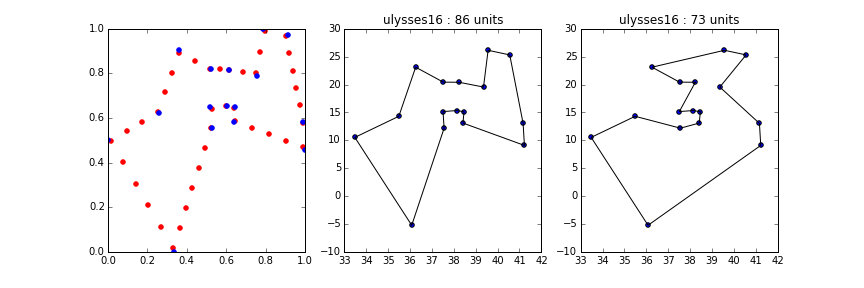
\includegraphics[scale=0.45]{figs/ulysses16}
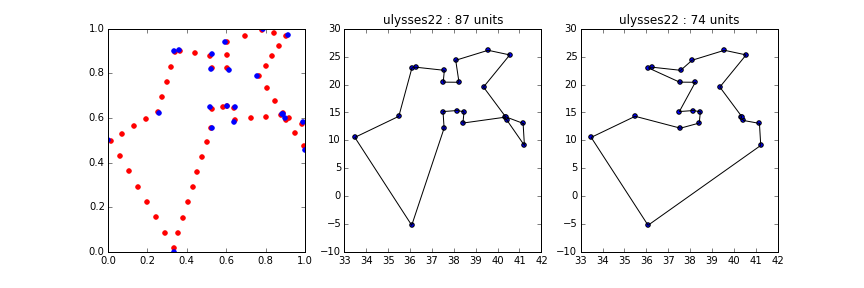
\includegraphics[scale=0.45]{figs/ulysses22}
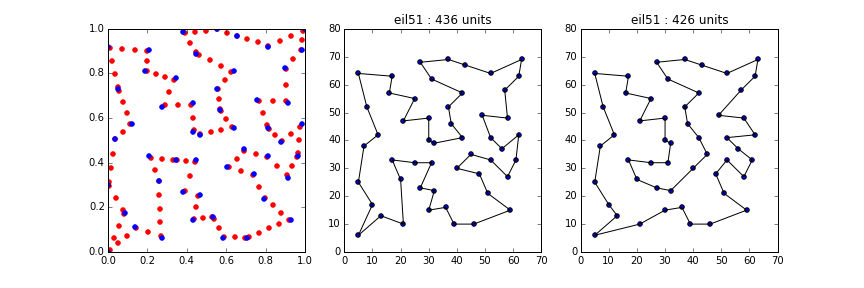
\includegraphics[scale=0.45]{figs/eil51}
 \end{center}
\end{figure}


\begin{figure}[!htb]
\begin{center}
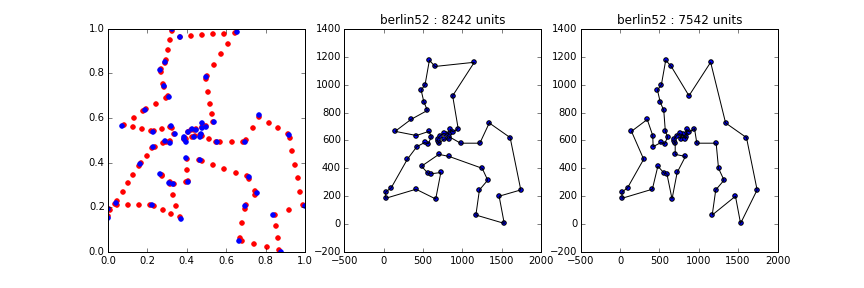
\includegraphics[scale=0.45]{figs/berlin52}
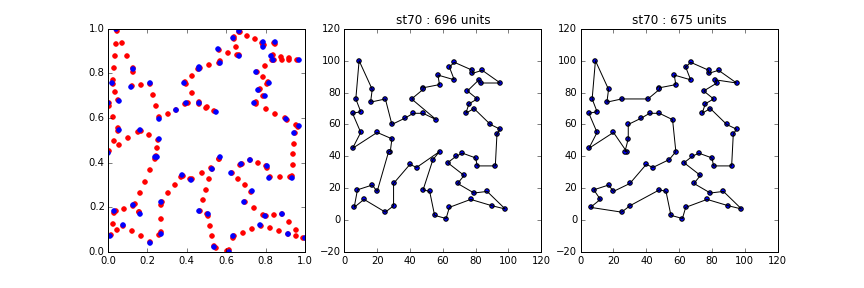
\includegraphics[scale=0.45]{figs/st70}
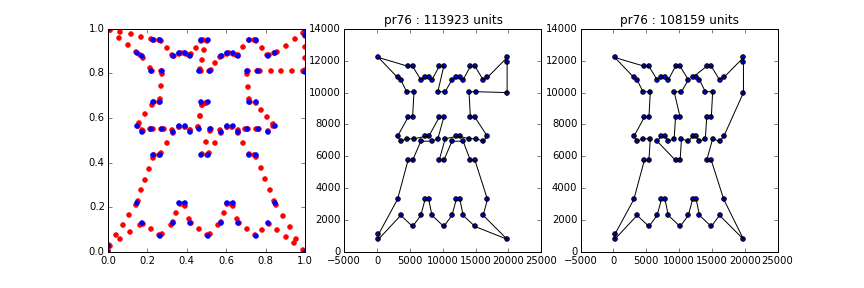
\includegraphics[scale=0.45]{figs/pr76}
 \end{center}
\end{figure}

 


\begin{figure}[!htb]
\begin{center}
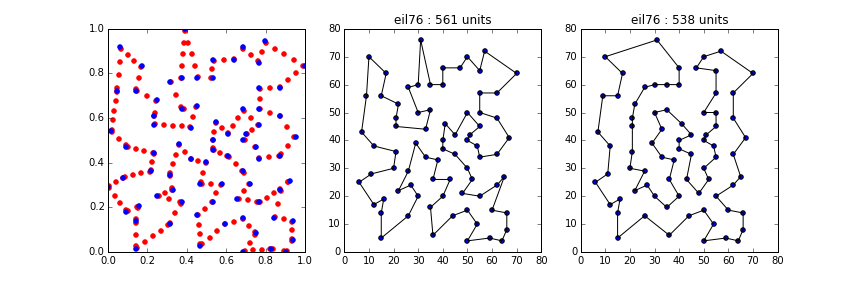
\includegraphics[scale=0.45]{figs/eil76}
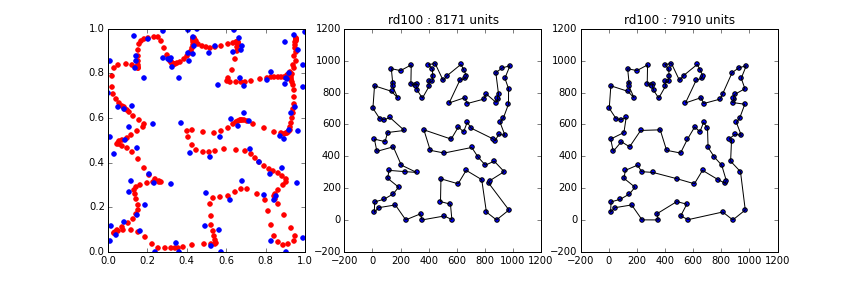
\includegraphics[scale=0.45]{figs/rd100}
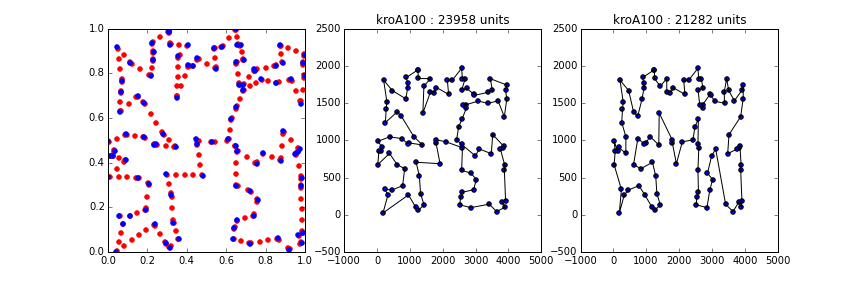
\includegraphics[scale=0.45]{figs/kroA100}

 \end{center}
\end{figure}


\begin{figure}[!htb]
\begin{center}
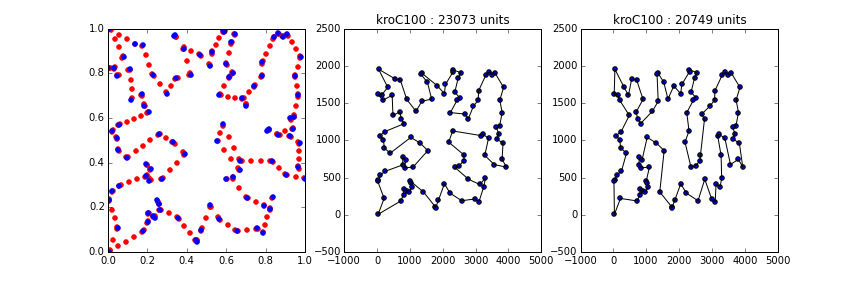
\includegraphics[scale=0.45]{figs/kroC100}
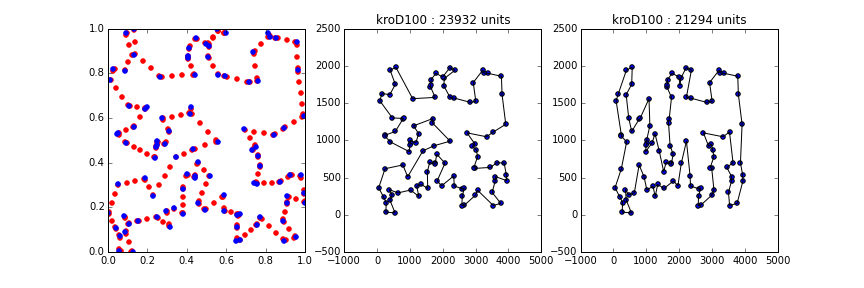
\includegraphics[scale=0.45]{figs/kroD100}
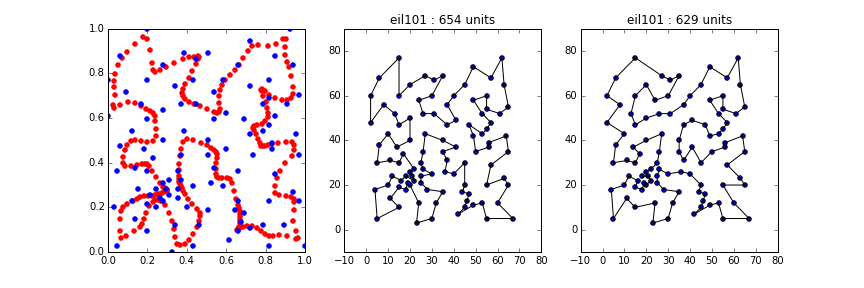
\includegraphics[scale=0.45]{figs/eil101}
 \end{center}
\end{figure}


\begin{figure}[!htb]
\begin{center}
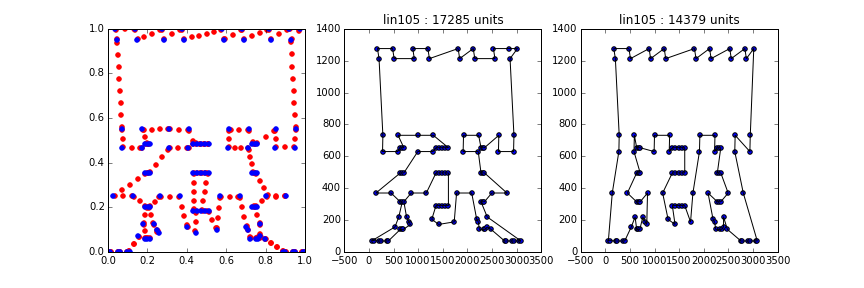
\includegraphics[scale=0.45]{figs/lin105}
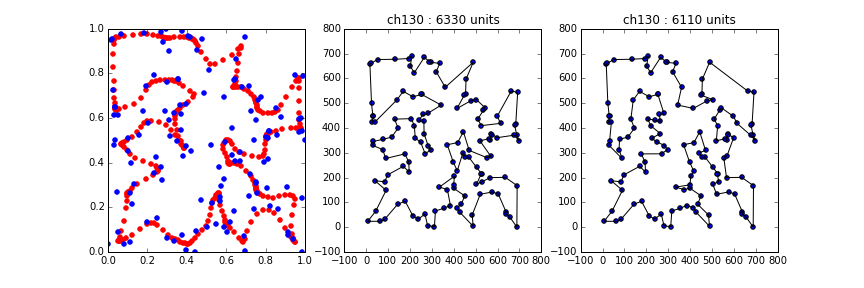
\includegraphics[scale=0.45]{figs/ch130}
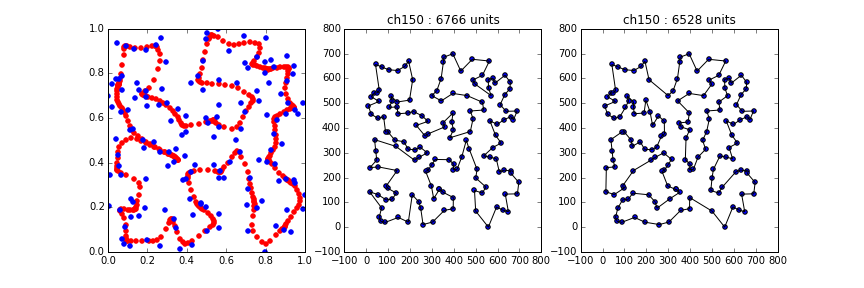
\includegraphics[scale=0.45]{figs/ch150}
 \end{center}
\end{figure}


 


\end{document}


